
%!TEX TS-program = xelatex
\documentclass[]{friggeri-cv}
\usepackage{afterpage}
\usepackage{hyperref}
\usepackage{color}
\usepackage{xcolor}
\usepackage[skins]{tcolorbox}
\hypersetup{
    pdftitle={},
    pdfauthor={},
    pdfsubject={},
    pdfkeywords={},
    colorlinks=false,       % no lik border color
   allbordercolors=white    % white border color for all
}
\addbibresource{bibliography.bib}
\RequirePackage{xcolor}
\definecolor{pblue}{HTML}{0395DE}

\begin{document}
\header{Lo\"{i}c}{Dutrieux}
      {Geo-Information Specialist}
      
% Fake text to add separator      
\fcolorbox{white}{gray}{\parbox{\dimexpr\textwidth-2\fboxsep-2\fboxrule}{%
.....
}}

% In the aside, each new line forces a line break
\begin{aside}
% TODO: Age, nationality could also be added here
    ~
    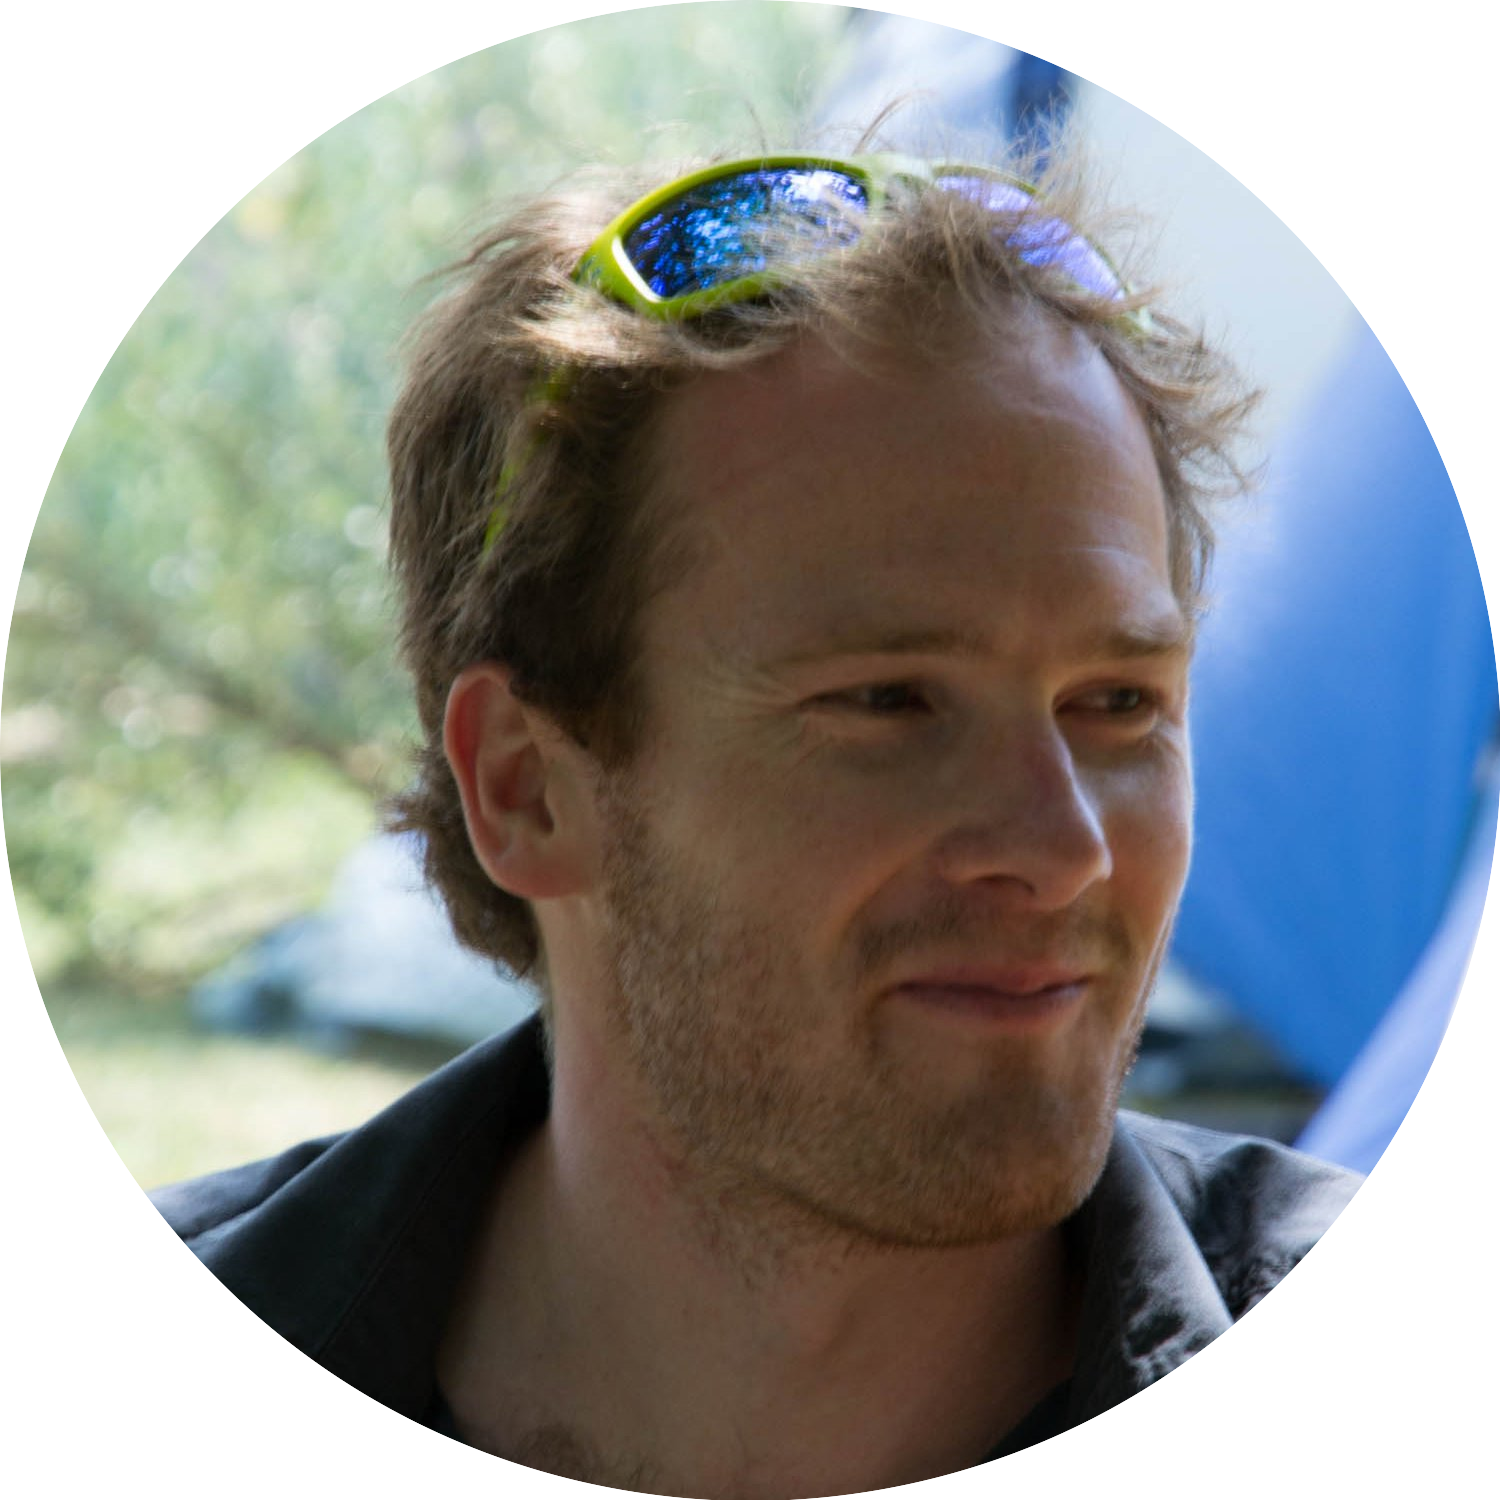
\includegraphics[width=2.5cm]{img/loic_circle.png}
    ~
  \section{Address}
    Sportstraat 52,
    6707GJ, Wageningen, Netherlands
    ~
  \section{Tel \& Skype}
    +31 612 025 297
    loic.dutrieux
    ~
  \section{Mail}
    \href{mailto:loic.dutrieux@gmail.com}{\textbf{loic.dutrieux@}\\gmail.com}
    ~
  \section{Web}
    \href{http://www.loicdutrieux.com}{loicdutrieux.com}
    \href{https://github.com/dutri001}{github.com/dutri001}
    ~
  \section{Programming}
    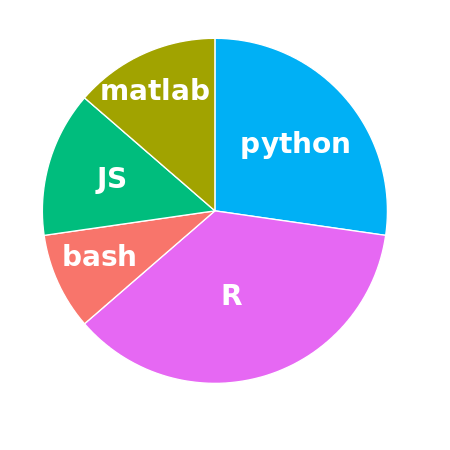
\includegraphics[width=3.5cm]{img/programming.png}
    ~
  \section{Tools and software}
  % TODO: OTB?
    \textbf{Linux}
\includegraphics[scale=0.40]{img/4stars.png}
    \textbf{Git}
\includegraphics[scale=0.40]{img/4stars.png}
    \textbf{QGIS}
\includegraphics[scale=0.40]{img/4stars.png}
    \textbf{GDAL}
\includegraphics[scale=0.40]{img/4stars.png}
    ~
  \section{Personal Skills}
    % 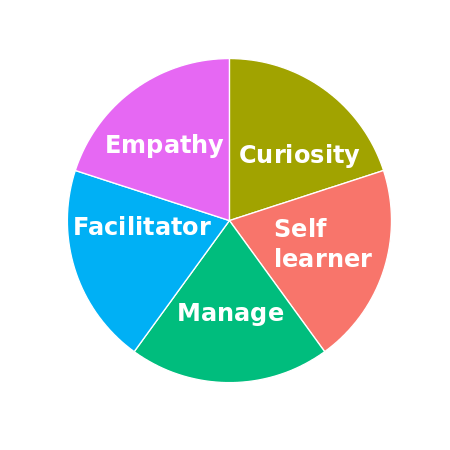
\includegraphics[width=3.5cm]{img/personal.png}
    \textbf{Empathy}
    \textbf{Curiosity}
    \textbf{Self learner}
    \textbf{Manager}
    \textbf{Facilitator} 
    ~
\end{aside}

% TODO: Would be nice to start here with a profile section section: a 4 lines description of who I am and what are my interests 

\section{Experience}
\begin{entrylist}
  \entry
    {02/12 - Now}
    {PhD Researcher}
    {Wageningen University, The Netherlands}
    {Research on forest dynamics and biodiversity mapping from satellite images time-series, development of open source toolboxes for spatial analysis, course design \& teaching, linux systems administration, active participation in large collaborative EU funded research project.\\}
  \entry
    {09/11 - 02/12}
    {Research Assistant}
    {Wageningen University, The Netherlands}
    {Coordination of elaboration and writing of a collaborative FP7 proposal among 8 European partners, Research on Arctic vegetation dynamics.\\}
    % \entry
    % {06/10 - 04/11}
    % {Master Thesis}
    % {Mali, Benin, Netherlands}
    % {Master research on mapping water water productivity in rice systems using remote sensing, research design, field work, data analysis.\\}
    \entry
    {01/10 - 02/10}
    {Academic Consultancy - Team manager}
    {Wageningen University, The Netherlands}
    {Team manager for a Consultancy project supervised by Wageningen University and commissioned by WATEURF (Water and Turf – Efficiency and Use Reduction for the Future)\\}
    \entry
    {06/08 - 09/08}
    {Internship}
    {Ministry of Agriculture, Central Farm, Belize}
    {Design of a pressurized irrigation system to irrigate pastures at the experimental farm of the ministry of agriculture of Belize\\}
    \entry
    {2007 - 2009}
    {Mountain guide - Seasonal}
    {UCPA, self employed}
    {Leading groups through two mountain ranges in the French Alps}
\end{entrylist}

\section{Education}
\begin{entrylist}
  \entry
    {2011 - 2015}
    {PhD}
    {Wageningen University, The Netherlands}
    {Remote sensing, time-series analysis, ecology, algorithm development\\
    Post graduate courses: Efficient writing, statistics, forest ecology, global forest carbon policies, psychology of performance.\\
    Thesis on \emph{Remote sensing based mapping of tropical forests ecosystems and their dynamics.}\\}
  \entry
    {2009 - 2011}
    {MSc International Land and Water Management}
    {Wageningen University, The Netherlands}
    {Main subjects: Irrigation, hydrology, water management, social aspects of land and water management \\
    Major thesis on \emph{Mapping water productivity of rice using remote sensing}\\
    Minor thesis on \emph{Vegetation dynamics in the Arctic from Moderate resolution remote sensing time-series}\\}
  \entry
    {2007 - 2011}
    {Master degree in Environment and Agriculture Engineering}
    {Ecole Supérieure d'Agriculture d'Angers, France}
    {Main subjects: Agronomy, landscape ecology, spatial analysis, Geopolitics, Management and Marketing}
  \entry
    {2005 - 2007}
    {DUT (\textit{French professional Bachelor}) Biology and Environmental Engineering}
    {IUT de Digne-Les-Bains, France}
    {Main subjects: Hydro-biology, Waste Water Management, Thermodynamic}
\end{entrylist}

\section{Contributed open source projects}
    \textbf{bfastSpatial}: \textit{Set of utilities and wrappers to perform change detection on satellite image time-series (Landsat and MODIS)}\\
    \\
    \href{http://geoscripting-wur.github.io/}{\textbf{GeoScripting course}}: Open source master course on scripting for Geo-Information Science taught at Wageningen University\\
    \\
    Regular contributor to the \href{https://stat.ethz.ch/mailman/listinfo/r-sig-geo}{R-SIG-Geo} mailing list

\begin{aside}
~
~
~
  \section{Places Lived}
    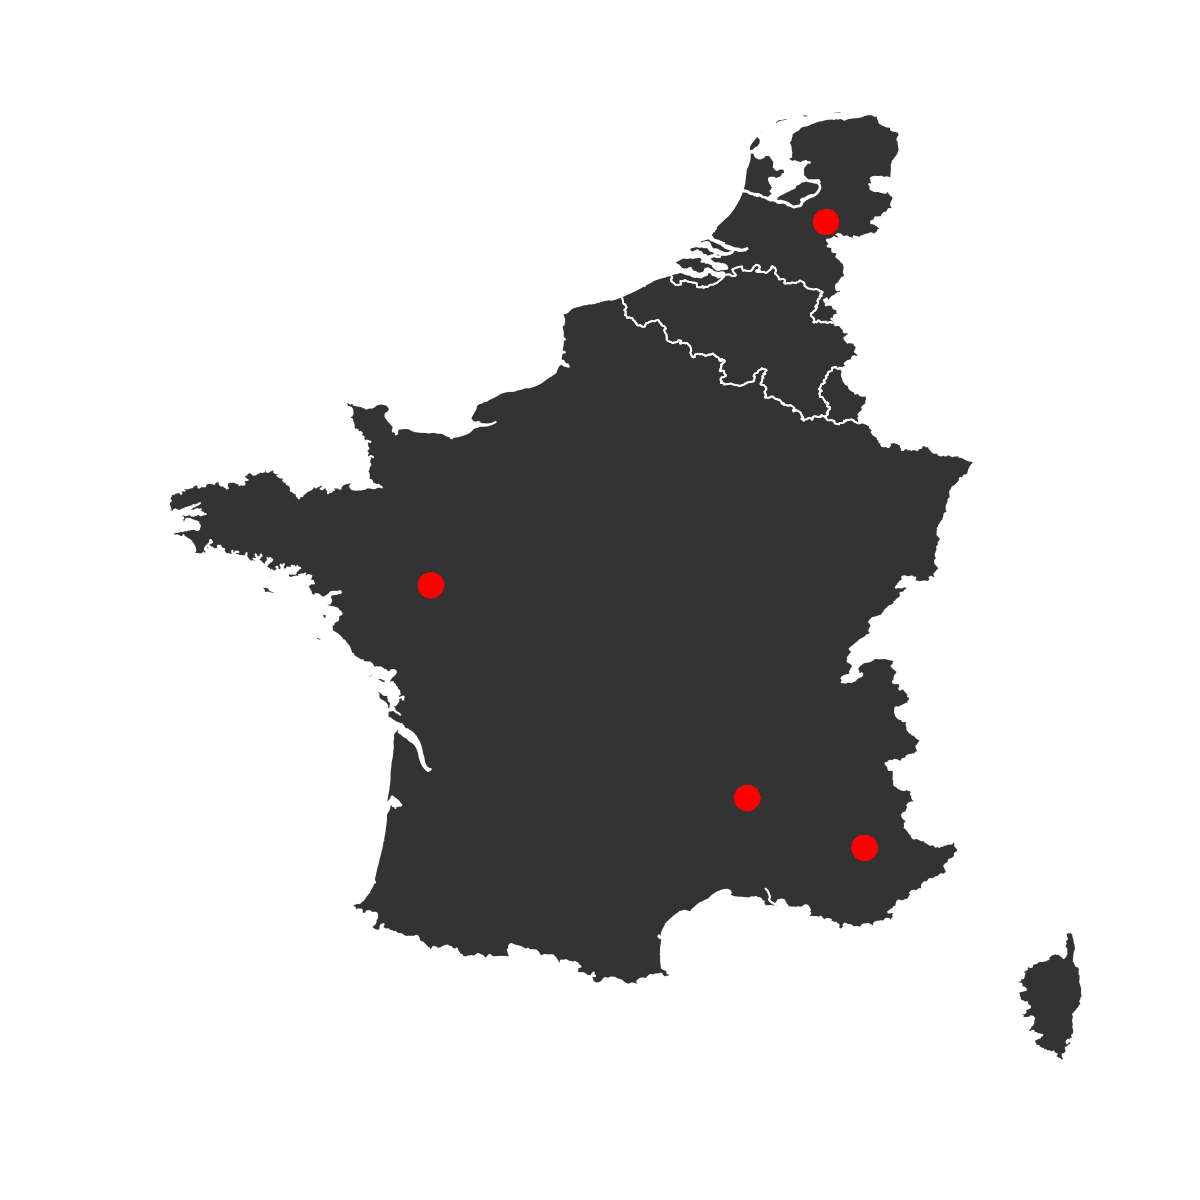
\includegraphics[width=3.5cm]{img/map.png}
    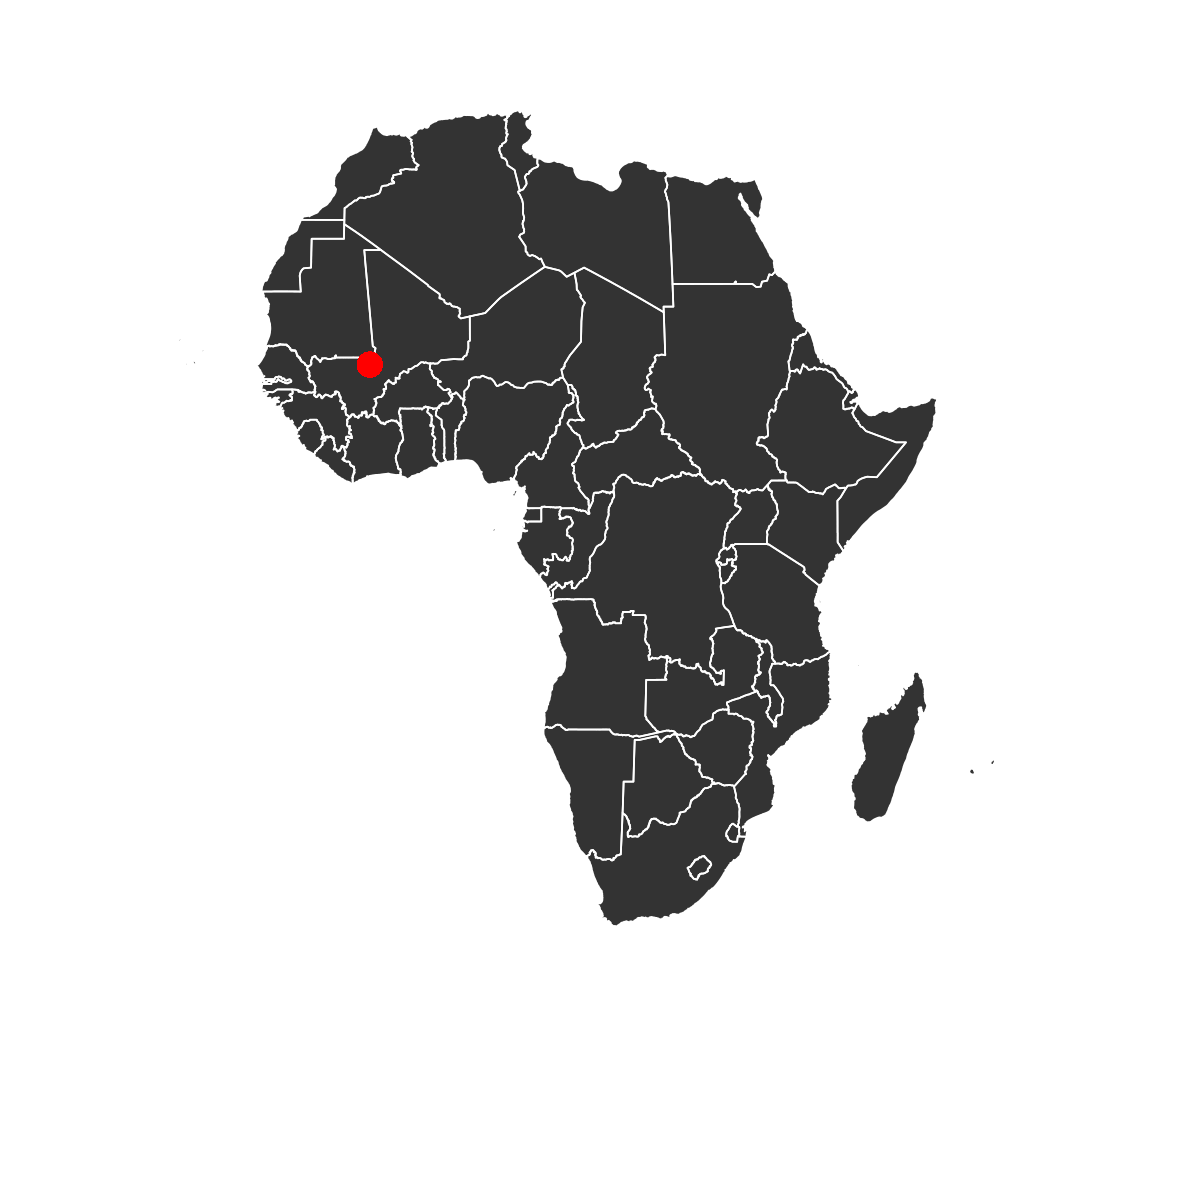
\includegraphics[width=3.5cm]{img/mapAfrica.png}
    ~
  \section{Languages}
    \textbf{English}
\includegraphics[scale=0.40]{img/4stars.png}
    \textbf{French}
\includegraphics[scale=0.40]{img/5stars.png}
    \textbf{Spanish}
\includegraphics[scale=0.40]{img/2stars.png}
\end{aside}

% TODO: \section{Self taught subjects}
\section{Honors and Awards}
	\textbf{Oustanding Student Paper Award of the American Geophysical Union (AGU)}\\
	Talk given at the AGU fall meeting, San Francisco, 2016

\section{Scientific work}
    Dutrieux, L. P., Jakovac, C., Latifah, S., Kooistra, L. (2016)\\
    \textbf{Reconstructing land use history from Landsat time-series. Case study of a swidden agriculture system in Brazil}\\
    \textit{International Journal of Applied Earth Observation and Geoinformation}\\
    \\
    Dutrieux, L. P., Verbesselt, J., Kooistra, L., Herold, M. (2015)\\
    \textbf{Monitoring forest cover loss using multiple data streams, a case study of a tropical dry forest in Bolivia.}\\
    \textit{ISPRS Journal of Photogrammetry and Remote Sensing}\\
    \\
    Dutrieux, L. P., Poorter, L., Equihua, J., Ascarrunz, N., Herold, M., Pe\~{n}a-Claros, M., Roerink, G., Toledo, M., Kooistra, L. (\textit{in review})\\
    \textbf{Country wide mapping of forest diversity and structure by combining forest inventories with remote sensing.}\\
    \\
    Dutrieux, L. P., Bartholomeus, H., Herold, M., Verbesselt, J. (2012)\\
    \textbf{Relationships between declining summer sea ice, increasing temperatures and changing vegetation in the Siberian Arctic tundra from MODIS time series (2000–11).}\\
    \textit{Environmental Research Letters}\\


\begin{flushleft}
\emph{November 29th, 2015}
\end{flushleft}
\begin{flushright}
\emph{Lo\"{i}c Dutrieux}
\end{flushright}

\end{document}
